\chapter{Introduction}
\label{chap:intro}

\section{Overview}

Understanding the processes that go into the formation and evolution of stars and stellar systems is crucial in the study of the chemical composition and structure formation of the universe. Stars are also central to the formation of planetary systems and are where the ingredients for life were formed. The energy provided by stars is necessary to maintain the life on planets. The study of the formation and evolution of the Sun, and more generally that of stars, would help us understand more about our origin and the future of our Solar System. This is one of the main reasons that the study of stellar structure and evolution has been a central topic in astronomy and astrophysics for decades.    
 
In order to completely understand the formation and evolution of galaxies from early universe to the current epoch, the knowledge of the formation of stars is necessary. Star formation determines the structure and evolution of galaxies, by transforming gas into stars. Moreover, the knowledge of star formation is essential to understanding the origin of planetary systems. The physical process of star formation is naturally complex. Therefore, the basis for a theory of star formation requires a strong foundation of empirical data or observations.

In a galaxy like our own, star formation begins with condensation of giant molecular clouds (GMCs, $\sim 10^7$ M$_{\odot})$ in the interstellar medium (ISM) which is due to gravitational instabilities. The interplay of turbulence and magnetic field with self-gravity is believed to be responsible for the formation of clumps within GMCs. Some of these clumps develop into self-gravitating cores, which have a similar distribution to stellar initial mass function (IMF) while turbulence and magnetic field play central roles in defining this distribution. Numerical simulations have shown that magnetic fields in the cores become supercritical and collapse\citep{Basu97}. In the process of  collapsing, an accretion disk is formed and significant magnetic flux is lost while the star also gradually loses its angular momentum. Powerful winds are magnetocentrifugally driven from the surface of the disk and turn into a jet-like flow due to magnetic hoops stresses \citep{Shu94}. This wind flows from the protostellar core and sweeps up gas into a massive molecular outflow. Massive stars form from massive cores, which are highly energised. These stars are highly luminous, therefore, they ionize their surrounding gas into HII regions. GMCs lose much of their original mass due to photo-evaporation. Most of the mass lost returns to the diffuse interstellar medium and completes the cycle of star formation, which then starts a new cycle (see \cite{McKee07} for more detail).  

  
The study of star formation has been an ongoing process and extends into the present era. The physical processes of star formation can be studied by direct observation. For more than 50 years, the numerical simulations, the empirical and theoretical laws, which describe the star formation rate have been investigated; nevertheless, their results have never been precise. Formation of stars is a complicated process. Various phenomena affect the collapse of molecular clouds and star formation which include the environment of the star-forming region, chemical compositions, the initial mass distribution of gas, gas accretion and cooling, H$_2$ formation, etc. Thus to fully understand this intricate process, many theories have been proposed and numerical simulations are carried out.

Despite the complex physical properties, fortunately there are empirical scaling laws to relate the star formation to other properties of galaxies. The most well-known of these scaling laws is the relation between the surface density of the star formation rate (SFR) and the gas surface density, which is known as the Kennicutt-Schmidt (KS) law \citep{Schmidt59, Kennicutt98a}. Similar to KS law, another scaling relation was derived which is a linear scaling between the total SFR and the mass of molecular gas (refer to the review by \cite{Elmgrenn11}). More recently, \cite{Shi11} derived another scaling relation, which relates the surface density of the SFR of galaxies to both gas surface density and the stellar mass.  

In this paper, we present the observational review of measuring the star formation rate and other properties that affect measuring and scaling the SFR in nearby galaxies. In $\S2$ we discuss measuring the star formation rate. A discussion of the ISM is presented in $\S3$, followed by a discussion of the measurement of the stellar mass in $\S4$. In $\S5$ the KS law and the models for scaling the star formation rate are introduced. The current issues about KS law and the present project are discussed in $\S6$. 

%-----------------------------------------------------
% Chapter: SFR
%-----------------------------------------------------
\section{Star Formation Rate}
\label{chap:sfr}

Understanding formation of stars leads to understanding galaxy formations. Characterisation of the star formation processes, such as the total SFR and the initial mass function of a galaxy, is necessary in examining its structure formation \citep{McKee07}. The main problem is that measuring the SFR is not trivial and depends on the galaxy morphology, metallicity, IMF, the spatial resolution of a target system, etc. There is a large number of review papers in the literature on how stars form and how their formation is traced. From a theoretical perspective, one can refer to the classic picture of the theory of star formation as reviewed by \cite{Shu87} and more recently by \citep{McKee07}. From an observational standpoint, star formation is discussed by \cite{Kennicutt98b, Kewley02, Bell03, Calzetti07, Calzetti08, Calzetti10, Calzetti13, Kennicutt07, Kennicutt09, Boquien10, Hao11, Kennicutt12}.

Many groups have been trying to define a technique to calibrate emission from the newly-born, hot and massive ``€œO"€ and ``€œB"€ stars to the rate at which stars are being formed. Emission from the young massive stars are normally used as a tracer of the current SFR. Using luminosity of massive stars makes sense if one considers that star formation rate has remained largely constant during the timescale probed by the specific wavelength which is being used as the tracer. The number of massive stars can be used to extrapolate the total number of the high and low mass stars that are formed in a given star-forming region. To do so, the stellar IMF must be known. However, knowing the Stellar IMF is not enough. To have a reliable SFR indicator, the stellar IMF must be fully sampled, which means that in the highest-mass bin at least one star is formed and all other mass bins have one or more stars (see section ~\ref{sec: imf}).

The ``O"€™ and ``€œB"€ stars can be observed by both using direct and indirect emission from stars; thus the SFR indicators are categorized based on these methods of observation. In the direct method, the SFR indicators can be probed by the ultraviolet (UV), optical, and near-infrared (NIR) emissions, while for probing the stellar light obscured by dust, mid/far-infrared emission is used. The ionizing photons are used in the indirect method. They are emitted by massive stars and traced by the ionized gas \citep[e.g.,][]{Calzetti04, Calzetti07}. In principle, the SFR is traced by the UV emission, the optical light, near-IR and radio wavelengths, hydrogen recombination lines, forbidden metal lines, and also in the sub-millimetre range by using the Bremsstrahlung emission. Moreover, high mass binaries, massive stars and supernova explosions produce X-ray emissions which can be used as a tracer of star formation. Each of these tracers has some systematic errors, and one should decide which of these methods are more precise for a given system. for example using dust IR emission as an indicator is not precise in dwarf galaxies with small amounts of the gas, although still errors from dust extinction and attenuation must be considered (see section ~\ref{sec: ism}).


\subsection{Stellar Initial Mass Function}
\label{sec: imf}
One of the most fundamental and difficult questions that a complete theory of star formation must answer is the initial mass function. In order to determine the SFR from calibrated photometry data, it is necessary to know the IMF. Most problems in modern astrophysical studies regarding the origin and evolution of stars and galaxies can be solved by varying an IMF \citep{Bastin10}. \cite{Salpeter55} empirically derived the IMF from the observed stellar luminosity function of the Solar neighbourhood \citep{Shu87}. He introduced a power-law IMF of the form:

\begin{equation}
\label{equ: salp}
\Phi (\log M) = dN / d \log M \propto M^{-\gamma }
\end{equation} 
where M is the mass of a star, $\gamma$ is the power index, and N is the number of stars in some logarithmic mass range $\log M + d\log M$. 

In the late 70s, it was recognised that using the single power-law IMF over all stellar masses is not a correct assumption \citep{Kroupa93, Bastin10}. Since then, many groups have studied the IMF and found different power laws for it (Fig.{~\ref{fig: imf}} ). Most SFR calibrations have the same assumption that the IMF is constant across all environments which is adopted from the standard IMF of \cite{Kroupa01}:

\begin{align}
\chi (M) = dN/dM = A M^{-1.3}    \quad    (0.1 \le M(M{\odot}) \le 0.5)\\                  
           = 0.5 A M^{-2.3}    \quad    (0.5 \le M(M{\odot}) \le 100)
\end{align}
where $\chi(M)$ is the number of stars between masses $M$ and $M+dM$. Although the Salpeter IMF produces more low-mass stars then the Krupa IMF, they produce almost the same number of the high mass stars. Therefore, the SFR calibrations, which mostly trace massive stars in galaxies, based on the Kroupa IMF and Salpeter IMF can be converted to one another by multiplying the calibration's constant by 1.6 \citep{Calzetti13}. \cite{Bastin10} reviewed  the IMF  by using many observational results and showed that the IMF is constant and universal, although there are uncertainties in different mass bins especially at the high mass end.

\begin{figure}[h]
\label{fig: imf}
\centering
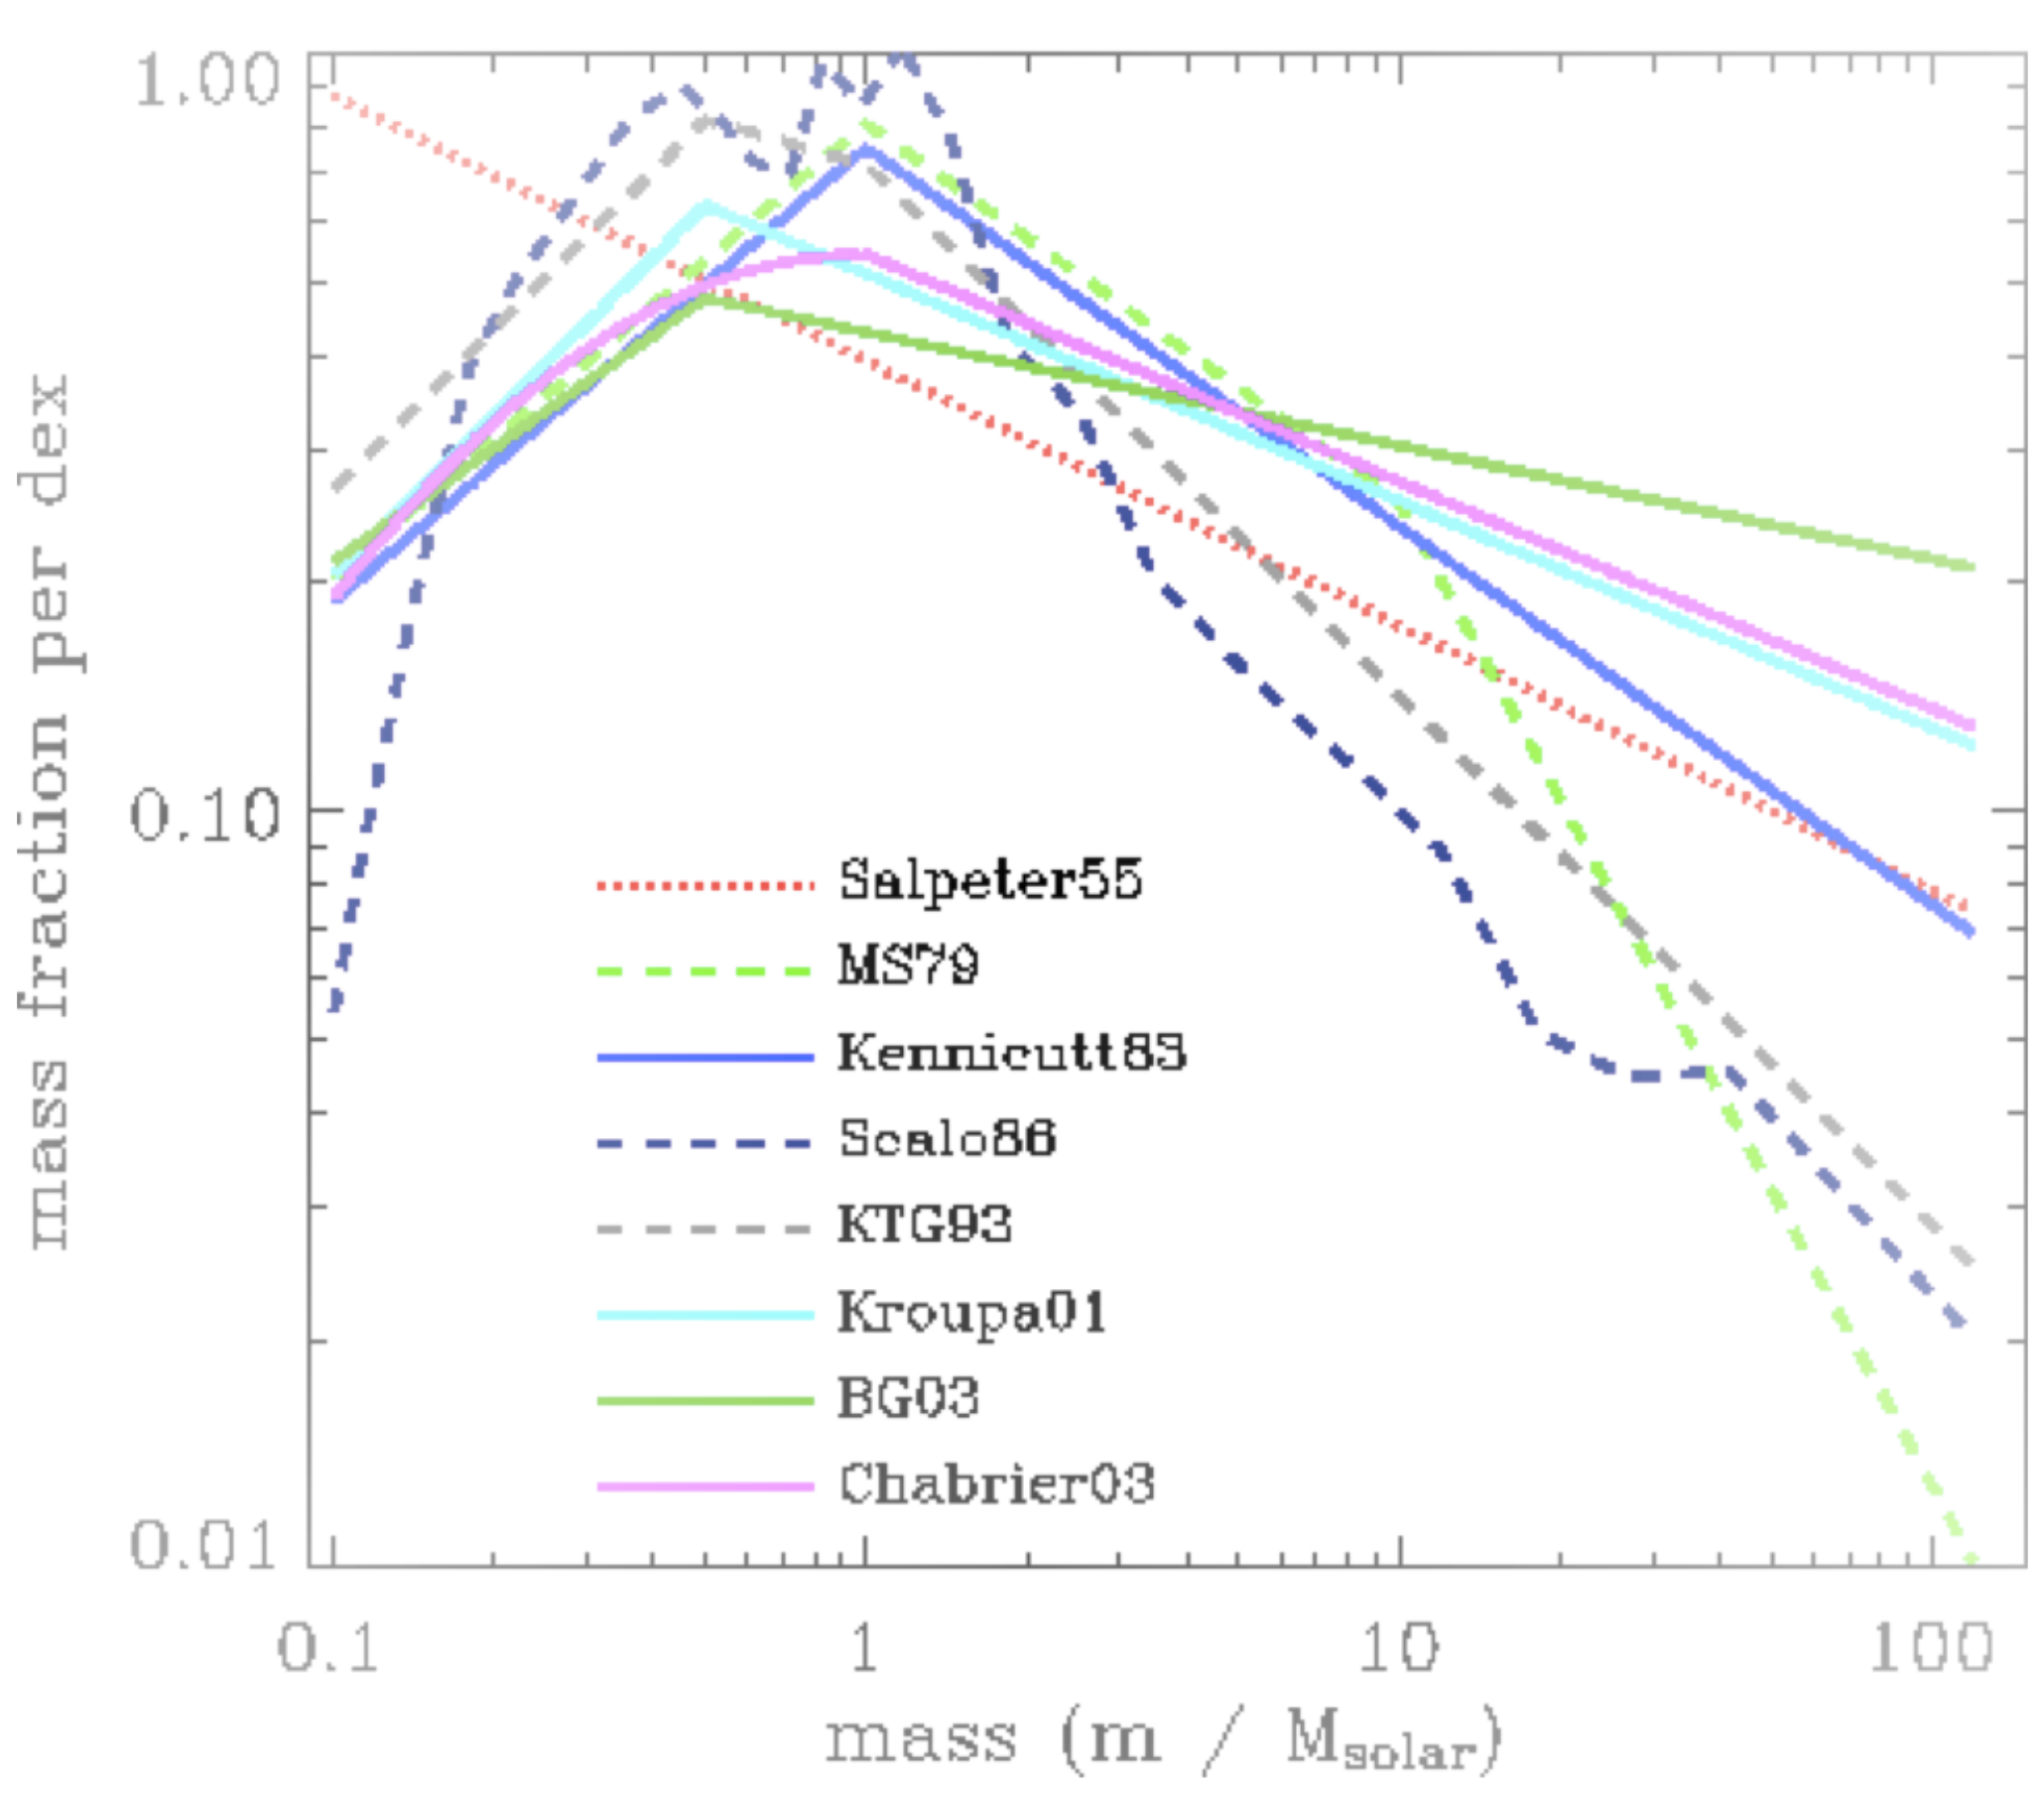
\includegraphics[width=16cm]{../image_intro/imf}
\small
\caption{Comparing the IMFs by plotting the mass fraction per dex versus mass that is normalized so that the integral under each curve is unity. The mass ranges from 0.1 to 120 M$_\odot$. Adopted from \cite{Baldry03}}
\end{figure}


The careful measurement of the IMF is a key to understanding the SFR. In distant galaxies, only massive stars can be detected; therefore, the IMF must be measured to include all stellar mass ranges in the SFR calibrations. To show the impact of the different IMF assumptions on the SFR calibrations, \cite{Calzetti13} used two different IMFs and derived the SFR calibrations with these new assumptions. Adopting a modified \cite{Kroupa01} IMF, with its maximum stellar mass set to 30 M$_{\odot}$ instead of 100 M$_{\odot}$, changes the SFR calibration constant by factors ranging from 1.4 to 5.6 for different SFR indicators (Table {~\ref{table1}}).  

\subsection{SFR Indicators}

One of the main issues to study distanced galaxies is the calibration of SFR indicators \citep[e.g.,][]{Lee10}. Calibration of SFR indicators can be affected by differences in star formation history (SFH), metallicity, distribution of stellar population and dust between different galaxies \citep{Calzetti13}. Depending on spatial resolution of the system one can divide star formation indicators into two categories: resolved and unresolved star formation indicators.

\subsubsection{Resolved Star Formation Indicators}
The most direct way to measure the SFR and trace recent star formation is counting individual objects \citep{Kennicutt12}. These objects mostly have certain ages and usually are referred to as young stellar objects (YSOs). Counting YSOs is a method used for calculating star formation in molecular clouds within $0.5- 1$ kpc of the Solar System. The number of YSOs can be converted to SFR using: 

\begin{equation}
SFR(YSO) = N_{yso} <M> \ \tau 
\end{equation}
where N$_{yso}$ is the number of YSOs, $<$M$>$ is the mean mass of YSO which depends on the stellar initial mass function (IMF; see section~\ref{sec: imf}), and $\tau$ is the lifetime of the YSO considering some uncertainly $\tau \sim 2$Myr \citep{Evans09}. The SFR(YSO) is in the unit of M$_{\odot}$yr$^{-1}$. Due to observational difficulties, this method can only be applied to the Milky Way and the Solar neighbourhood. 

In theory, for any system with high enough spatial resolution ($\sim 0.5- 1$ kpc), counting YSOs can be used as a tracer of the star formation. However, considering the limited capabilities of the present instrumentations, YSOs in most regions beyond the Magellanic clouds can not be resolved. Therefore, most studies use the emission from the ``O" and ``B" stars as tracer of the SFR. Another method to measure the SFR is by looking at the colour-magnitude diagram (CMD) of star-forming regions. \cite{Kennicutt12} discusses the new progress made in the spatially-resolved mapping of CMDs to reproduce the spatially and age-resolved maps of star formation in nearby galaxies. More detailed studies of CMDs are not in the scope of this paper; for more information, one can refer to \citep{Kennicutt12}. 

\subsubsection{Unresolved Star Formation Indicators}
 In star-forming regions farther away than the Magellanic clouds, spatial resolution is not high enough to find all the YSOs. In unresolved systems, luminosity, which is either single band or integrated over some wavelength range, is used as an SFR indicator. This method is used to find continuum or line emission at some wavelengths that are sensitive to the young massive stars \citep[e.g.,][]{Kennicutt98b, Calzetti13}. \cite{Kennicutt98b} reviewed calibrations of star formation tracers. He calibrated luminosity for measuring the SFR in specific wavelengths using relations between the SFR per unit mass or per unit luminosity and the integrated colour of the system provided by synthesis models \citep[e.g.,][]{Bruzual93}. 

In unresolved systems, the SFR indicators can be divided into local and global SFR indicators. The global SFR indicators are defined for entire galaxies; therefore, they are luminosity-weighted averages across local star formation history and the physical condition inside each galaxy. While local calibration is used for regions within a galaxy, on a scale of sub-galaxy \citep[e.g.,][]{Zhu08, Kennicutt09, Boquien10, Boquien11, Hao11}. The limitations in the spatial resolution of the data on the one hand, and the broader applicability of distant galaxy populations on the other, have brought more attention to the calibrations of global SFR compared with the local SFR calibrations that had been done in the past. Yet, because of its ability to trace the physical processes of the star formation, local SFR calibration is becoming increasingly important \cite{Calzetti13}.

The following subsections describe some SFR indicators in more detail. In this paper, we categorise the SFR indicators into tracers based on single-band emission and those that are based on the multi-band emission. For each category, we discuss if a calibration can be used as local or global and also describe their differences.  

\subsubsection*{SFR Indicators Based on the Single-Band Emission}

In order to derive the conversion between the luminosity in specific wavelengths and the SFR, synthesis models are used \citep{Kennicutt98b}. General form of a SFR calibration using single-band emission is: 
\begin{equation}
\label{equ: sfrsingle}
SFR(\lambda)= CL(\lambda)
\end{equation}
where SFR is in units of M${_\odot}$yr$^{-1}$, $L(\lambda)$ is luminosity in erg/s at the wavelength $\lambda$, and C is the constant derived from stellar population models (Starburst99, \cite{Leitherer99}). The constant, C, can vary for different emission, mass ranges of the stellar IMF, and the timescale $\tau$ over which star formation needs to remain constant. Table~\ref{table1} from \cite{Calzetti13}, summarises the changes in the constant of the calibration. 

\begin{table}[ht]
\caption{Luminosity-to-SFR calibrations adapted from \cite{Calzetti13}\label{table1}}
\centering
\begin{tabular}{ c c c }
\hline\hline
Luminosity\footnotemark{} & C\footnotemark{} & Assumptions\footnotemark{}\\
\hline
L(UV) & $3.0 \times 10^{(-47)} \lambda$ &$0.1 -100 M_{\odot}, \tau \ge 100 Myr $\\
L(UV) & $4.2 \times 10^{(-47)} \lambda$ &$0.1 -30 M_{\odot}, \tau \ge 100 Myr $\\
L(UV) & $4.3 \times 10^{(-47)}\lambda$ &$0.1 -100 M_{\odot}, \tau = 10 Myr $\\
L(UV) & $1.0 \times 10^{(-46)}\lambda$ &$0.1 -100 M_{\odot}, \tau = 100 Myr $\\
L(TIR) & $1.6 \times 10^{(-44)}$ &$0.1 -100 M_{\odot}, \tau = 100 Myr $\\
L(TIR) & $2.8 \times 10^{(-44)}$ &$0.1 -100 M_{\odot}, \tau = 100 Myr $\\
L(TIR) & $4.1 \times 10^{(-44)}$ &$0.1 -30 M_{\odot}, \tau = 100 Myr $\\
L(TIR) & $3.7 \times 10^{(-44)}$ &$0.1 -100 M_{\odot}, \tau = 100 Myr $\\
L(TIR) & $8.3 \times 10^{(-44)}$ &$0.1 -100 M_{\odot}, \tau = 100 Myr $\\
L(H${\alpha}$) & $5.5 \times 10^{(-42)}$&$0.1 -100 M_{\odot},  \tau \ge 6 Myr $\\
L(H${\alpha}$) & $3.1 \times 10^{(-41)}$&$0.1 -30 M_{\odot},  \tau \ge 10 Myr $\\
\hline
\end{tabular}
\end{table}
\footnotetext[1]{Luminosities are in erg/s and are given as $\nu L_{\nu}$.}
\footnotetext[2]{The constant C appears in equation~\ref{equ: sfrsingle}. For SFR(UV), the numerical value is multiplied by the wavelength $\lambda$ in $\AA$.}
\footnotetext[3]{Assumptions for mass range of the stellar IMF, which we adopt to have the expression derived by \cite{Kroupa01} (see section{~\ref{sec: imf}}), and for the timescale $\tau$.} 


One of the most common single-band wavelengths, which are used as an SFR indicator, is UV emission. UV emission can be an excellent tracer for the SFR due to the fact that the peak of emission for both ``O" and ``B" stars are in the UV part of the spectrum. Using spectral energy distribution (SED) from Starburst99, with solar metallicity and assuming \cite{Kroupa01} stellar IMF with the timescale of over 100 Myr, SFR can be measured as \citep{Leitherer99}
\begin{equation}
SFR(UV) = 3.0 \times 10^{-47}\lambda L(\lambda)
\end{equation}
where SFR(UV) is in M$_{\odot}$yr$^{-1}$, $\lambda$ is in $\AA$, and $L(\lambda)$ is in erg/s, while $\lambda$ is in the range of $(0.0912\mu$m $< \lambda < 0.3\mu$m). As shown in table ~\ref{table1}, with changes in the stellar ranges of the IMF, during timescales longer than 100 Myr, the calibration constant only decreases by a few percent. However, the calibration constant's changes for shorter timescales, are more significant \citep{Calzetti13}. The accuracy of the calibration constant is $\pm 15\%$ which can vary as a function of $\lambda$. The UV light can easily be absorbed or scattered by interstellar dust. Therefore, using the UV emission as a tracer might lead to underestimating of the SFR, if dust extinction corrections are not applied (\cite{Kennicutt12}; also see Section ~\ref{sec: ism}). 

Another single-band SFR indicator is the emission from hydrogen recombination lines. Ionizing photons emitted from young massive stars ionize the surrounding gas. Hydrogen recombination line emission, such as the Balmer series lines of H${\alpha}$ $(0.6563 \mu$m) and H${\beta}$ $(0.4861 \mu$m), which are located in the optical wavelength range, are among the most traditional SFR indicators \citep{Kennicutt98a}.  The relationship between the intensity of a hydrogen recombination line and the ionizing photon rate for a nebula is derived quantum mechanically. To have such results, the nebula must be optically thick to ionizing photons \citep{Osterbrock06}. Being optically thick makes almost all transitions more energetic than Ly${\alpha}$ to be absorbed and re-emited via Ly${\alpha}$ and longer wavelengths. This is why the H${\alpha}$ emission line strength is greater in optically thick environments. The relation between the SFR, the luminosity of the H$\alpha$ emission line and the ionizing photon rate is \citep[e.g.,][]{Osterbrock06, Kennicutt98b}:

\begin{align}
\label{equ: halpha}
SFR(H\alpha) = 5.5 \times 10^{-42}L(H\alpha) \\
                     = 7.4 \times 10^{-54}Q(H^{\circ})
\end{align}
where SFR(H$\alpha$) is in M$_{\odot}$ yr$^{-1}$, L(H$\alpha$) is in erg/s, and Q(H$^{\circ}$) which is the ionizing photon rate is in units of s$^{-1}$. The constant at the right-hand side of equation~\ref{equ: halpha} is the resulting coefficient for electron temperature T$_e=10000$K and density N$_e=100$ cm$^{-3}$ which is the normal case in the interstellar medium. All SFR indicators that use the ionization of hydrogen to trace the formation of massive stars are sensitive to the effects of dust. Dust extinction (Section ~\ref{sec: ism}) is the most important systematic error for calculating the SFR from hydrogen recombination line.The effects of dust must be measured and H$\alpha$ observations must be corrected or this could lead to underestimating the SFR \citep{Kennicutt98b}. 

Another nebular line, which is used as a tracer of the SFR is [OII]$\lambda$3727$\AA$. Although the luminosities of forbidden lines do not correlate with the ionizing atoms directly, their extinction has correlation with the H$\alpha$ emission. As a result, [OII] luminosity can be used as a tracer of the SFR through H$\alpha$ luminosity. \cite{Gallagher89} calibrated the SFR based on the [OII] luminosity by using a sample of 75 galaxies. Another calibration for this luminosity was derived by \cite{Kennicutt92}, which has a different calibration factor. In his review on the SFR, \citep{Kennicutt98b} averaged these calibrations and derived the following relation:
\begin{equation}
SFR(O[II]) = 1.4 \times 10^{-41} L(O[II])
\end{equation}  
where SFR(O[II]) is in M$_{\odot}$ yr$^{-1}$, L(H$\alpha$) is in erg/s. Although SFR (O[II]) is not as precise as the SFR(H$\alpha$), it is one of major SFR indicators in high redshift galaxies. In high redshift galaxies, H$\alpha$ emission line is out of optical bands, as a consequence, calibration of the strongest emission feature in the blue light (O[II]) as a SFR indicator is really useful \citep{Kennicutt98b}.


Since interstellar dust absorbs approximately half the starlight and re-emits in the infrared, the IR emission can be used to trace the SFR. The IR luminosity of a system depends not only on the amount of the embedded dust, but also on the heating rate provided by the stars. Since young stars heat the dust to higher mean temperatures than old stellar populations, to the first order the shape of the thermal IR SED depends on the starlight SED \citep{Helou86}. The fact that heating rate provided by the young stellar population is higher than the old stellar population indicates that dust heated by the former is more luminous and consequently its SED has peaked at shorter wavelengths (observationally $\approx 60  \mu$m) in comparison with the dust heated by old or low-mass stars.€“ Therefore, the IR wavelength is able to detect the emission from the young stellar population and be used as an SFR indicator.  

24 $\mu$m and 70 $\mu$m bands are two empirical single-band IR SFR calibrators. The use of these two bands depends on the type of the galaxy studied or the physical environment in different regions within the galaxy. Since the luminosity of a stellar population with constant star formation increases with time, the IR emission, which is used as a tracer of the emission of the stellar population, has different calibration constants in the case of a global (the entire galaxy SFR indicator) and a local indicator. That is because the global case includes the Hubble time integrated stellar population of a galaxy, while the other is calculated from regions with short star formation timescales such as: HII regions, large star-forming complexes, etc. \cite{Calzetti13}. Table ~\ref{table2} shows the constant C from equation~\ref{equ: sfrsingle} for 24 $\mu$m and 70 $\mu$m luminosities and for local (spatial scale $\sim500$ pc for 24$\mu$m band and spatial resolution less than $\sim 1$ kpc for 70 $\mu$m one) and global cases. 

\begin{table}[ht]

\caption{IR Luminosity to SFR calibrations \label{table2}}
\centering
\begin{tabular}{ c c c c }
\hline\hline
Luminosity\footnotemark{} & C & Assumptions & references\\
\hline
L(24)$^{0.885}_{local}$ & $1.31 \times 10^{(-38)}$ &$(1.10^{40} \le L(24) \le 3.10^{44})$& Calzetti et al. (2007)  \\
L(24)$_{global}$ & $2.04 \times 10^{(-43)}$ &$ (4.10^{42} \le L(24)  \le 5.10^{43})$& Calzetti et al. (2007) \\
L(70)$_{local}$ & $9.4 \times 10^{(-44)} $ &$(5.10^{40} \le  L(70) \le 5.10^{43})$& \cite{Li12} \\
L(70) $_{global}$& $5.9 \times 10^{(-44)}$ &$(L(70) \ge 1.4 \times 10^{42} $& \cite{Li10}\\
\hline
\end{tabular}
\end{table}  
 \footnotetext{Luminosities are in form of L($\lambda$) = $\lambda L(\lambda)$ in erg s$^{-1}$}
 %The SFR(70) calibration constant thus increases when going from whole galaxies to 1 kpc regions, i.e., for decreasing region sizes. According to the Li et al. (2012) this constant can be interpreted in terms of star formation timescale within each region (Fig.{~\ref{sfr70}}).
%\begin{figure}
%\label{sfr70}
%\centering
%\includegraphics[width=8cm]{sfr70}
%\caption{The calibration constant, C$_70$, between SFR and the 70$\mu $m luminosity, from equation~\ref{equ: sfrsingle}, as a function of the physical size of the regions used to derive the calibration. The filled red triangles are observed values from Li et al. (2010, 2012) and Calzetti et al. (2010), using both $Spitzer$ and $Herschel$ data. The black stars are from stellar population synthesis models, for constant star formation and a Kroupa (2001) IMF, in the stellar mass range of 0.1-100 M$_\odot$; the mean age of the population that best approximates the observed C70 values is shown. This figure is adapted from \cite{Calzetti13}.}
%\end{figure}

\subsubsection*{SFR Indicators Based on the Multi-Band Emission}

Despite the usefulness of having single-band SFR tracers, in many cases, one should be careful about the corrections due to dust effects, luminosity ranges, etc. Nowadays, thanks to large surveys, enormous data is available at different wavelengths for galaxies. This allows for combining the emission from different bands and finding new calibrations. Conversion between SFR and luminosities at different bands mostly helps avoiding problems regarding dust extinction or attenuation (see~\ref{sec: ism}). 

The simplest possible way to combine luminosities at different bands in order to convert them to SFR is through a linear relation, whose correlation with the SFR is empirically proved \citep{Kennicutt12}. There are studies that use a higher order polynomial relation to combine luminosities \citep[e.g.,][]{Buat05}; however, this discussion is out of the scope of this paper.

Integrating over the full wavelength range of the IR part of spectrum gives the total infrared (TIR) emission of a system, which can be used as an SFR indicator. As mentioned earlier, dust absorbs stellar radiation at all wavelengths; however, we only discuss radiation emitted from UV luminous stars. It must be noted that since there is no one-to-one mapping between IR and UV emission \citep{Calzetti13}, it is better to use the TIR emission as a tracer of the SFR instead of the IR single-band emission.
 
\cite{Draine07} modelled $Spitzer$ \citep{Wener04} data and found a calibration for the total infrared luminosity from photometry images instead of using IR SED. \cite{Boquien10} tested this calibration and found the modified version of calibration to estimate total infrared luminosity: 
\begin{equation}
L(\rm TIR) = 0.95L(PAH 8 \mu m) + 1.15L(24 \mu m) + L(70 \mu m) + L(160 \mu m)
\end{equation}
where $L = \nu L_{\nu}$ and $L_{\nu}$ is the luminosity  in erg/s at frequency $\nu$. \cite{Calzetti07} indicated that star formation rate calibration for a stellar population undergoing constant star formation over $\tau=100Myr$ is:
\begin{equation}
\label{sfr_tot_IR}
SFR(\rm TIR) = 2.8 \times10^{-44}L(\rm TIR)
\end{equation}
where SFR(TIR) is in M${\odot}$yr$^{-1}$, and L(TIR) is in erg/s. To do this calculation, it is assumed that stellar bolometric emission is completely absorbed and re-emitted by dust, i.e., $L_{star}(\rm bol)=L(\rm TIR)$.

The most common use of combining luminosities to trace the SFR is calibration of the SFR by combination of TIR measurements with both far and near UV observations, with the latter being more commonly used. This combination helps to avoid uncertainties from dust attenuation in FUV observations.
\begin{equation}
L_{FUV}(\rm corr) = L_{FUV}(\rm obs) + \alpha L_{\rm TIR}
\end{equation}
where the luminosities are $L = \nu L_{\nu}$ in erg/s, and the coefficient $\alpha$ depends on the bandpasses that are chosen for the UV and IR measurements. $\alpha$ is usually less than 1 because significant amounts of IR emission in many galaxies is from dust heated by older population stars \citep{Kennicutt12}. The coefficient $\alpha$ is calibrated both theoretically, using evolutionary synthesis models, and empirically, by using measurements of dust corrected SFRs (e.g., \cite{Hao11}. 

Another common method for using the multi-wavelength indicator for star formation is using H${\alpha}$ emission in combination with the $24\mu$m emission. This combination gives a more accurate dust-corrected estimate of the SFR \citep{Kennicutt09}:

\begin{equation} 
\label{equ: halphaplus24}
SFR = 7.9 \times 10^{-42}[L(H{\alpha})_{obs} + 0.020L(24)]
\end{equation}
where L(H${\alpha}$)$_{obs}$ is the observed H${\alpha}$ luminosity without correction for internal dust attenuation, given in the unit of erg/s. L(24) is the $24\mu$m IR luminosity in erg/s, and SFR is in M$_{\odot}$yr$^{-1}$.

\begin{table}[ht]
\caption{Multi-wavelength dust-corrected luminosities, adopted from \cite{Kennicutt12} \label{table3}}
\centering
\begin{tabular}{ c c}
\hline\hline
Combined luminosities\footnotemark{} & references\\
\hline
L(FUV)$_{corr}$=L(FUV)$_{obs}$ + 0.46L(TIR)& Hao et al. (2011)\\
L(FUV)$_{corr}$=L(FUV)$_{obs}$ + 3.89L(24$\mu$m)& Hao et al. (2011)\\
L(NUV)$_{corr}$=L(NUV)$_{obs}$ + 0.27L(TIR)& Hao et al. (2011)\\
L(NUV)$_{corr}$=L(NUV)$_{obs}$ + 2.26L(24$\mu$m)& Hao et al. (2011)\\
L(H$\alpha$)$_{corr}$=L(H$\alpha$)$_{obs}$ + 0.0024L(TIR)& Kennicutt et al. (2009)\\
L(H$\alpha$)$_{corr}$=L(H$\alpha$)$_{obs}$ + 0.020L(24$\mu$m)& Kennicutt et al. (2009)\\
\hline
\end{tabular}
\end{table}  
\footnotetext{Luminosities are in the form of L($\lambda$) = $\lambda L(\lambda)$ in erg s$^{-1}$}
 
Other combinations of luminosities that are used as tracers of the SFR are listed in table ~\ref{table3}. These composite SFR indicators also have systematic uncertainties; yet, it seems that there is good correlation between multi-band tracers and single-band tracers. Moreover, less uncertainty arises in this case than when using the single-band emission as a tracer \citep{Kennicutt09}. 

As mentioned in section ~\ref{sec: imf}, using different IMFs leads to having different SFR calibrations. From table~\ref{table1} it is clear that changing the IMF affects the H${\alpha}$ SFR calibration more than other SFR calibrations. This effect is more than four times larger than UV SFR calibrations because newly-formed stars having up to $\sim 5$ M$_{\odot}$ emit more strongly at UV radiations; however, significant amounts of ionising photons are produced by stars more massive than $\sim 20$ M$_{\odot}$. Furthermore, reaching an asymptotic value takes longer for more massive stars (10 Myr for the upper mass limit of 30 M$_{\odot}$ versus 6 Myr for 100 M$_{\odot}$). Therefore, changes in the H${\alpha}$ SFR calibration constant are more pronounced, while for UV and TIR calibration constants are fairly close to each other. On the other hand, using the mean stellar mass for the Kroupa IMF $(<$M$> \sim 0.6$ M$_{\odot})$ yields less than $10\%$ difference between using the upper mass limit of 100 M$_{\odot}$ and 30 M$_{\odot}$. As a result, calibrations derived with the mean stellar mass of a system are more accurate than those that are based on tracing the most massive stars \citep{Calzetti13}.
 
%%%%%%%%%%%%%%%%%%%%%%%%%%%%
%chapter: ISM
%%%%%%%%%%%%%%%%%%%%%%%%%%%%

\section{Interstellar Medium}

Interstellar medium (ISM) is referred to the space between stars in a galaxy, which is full of a thin hydrogen and helium gas and small amounts of heavier elements called metals. These elements can have neutral, ionized, or molecular forms and can be in gas phase or solid state. The gas and dust in the ISM are heated by interstellar radiation field and cool through a variety of line and continuum processes which usually depend on the local physical conditions. The ISM has a huge impact on the formation and evolution of stars. Since stars are born in the ISM and release their material into the ISM when they reach the end of their evolution, studying the ISM is essential in the understanding of the formation and evolution of stars.

Considering the effects of the ISM on studying the SFR is important for two main reasons. First, stars are born from the gas; therefore, for scaling the star-formation rate in a galaxy, knowledge on the amount of gas is necessary. The other impact is that gas and dust in the ISM absorb the UV or optical emission from stars and re-emit it in the IR, or scatter the stellar light. Thus for tracing the star-forming region, the effect of dust must be taken into account, otherwise the SFR might be underestimated. 

\subsection{Map of the ISM}
\label{sec: ismmap}


A map of the total gas in the ISM is produced by direct observations of the gas or using interstellar dust as a tracer. Neutral and molecular hydrogen are the most common elements in the ISM. Therefore, for producing the map of the total gas in galaxies, maps of these two components can be added together and multiplied by a constant factor to account for heavier elements which are mostly He. Another way to do the mapping is assuming that the ratio of total gas and dust is constant across a galaxy, and convert dust observations to the map of total gas.

\subsubsection{Direct Measurement of the Gas}

The surface density of gas in the ISM of galaxies can be measured by direct observation of the neutral and molecular hydrogen. This method can be promising provided that the spatial resolution of observational data is high enough; nonetheless, due to technical limitations, attaining enough spatial resolutions to resolve clouds is almost impossible. This problem shows itself for distant galaxies more than nearby galaxies. As a result, using this method is limited and has a lot of uncertainties. 
 
\subsubsection*{Molecular Clouds}

 The molecular form of hydrogen in the ISM has no permanent electric dipole moment, which makes it really hard to detect. H$_2$ molecules are located in cool and dense molecular clouds, but fortunately they are not the only component of the molecular gas. The second dominant component, helium, is a mono-atomic gas and has the same problem as hydrogen, but the molecular gas also contains heavier elements such as carbon and oxygen which are combined to form CO \citep{Bolato13}. 
 
CO has a weak permanent electric dipole moment and a ground rotational transition with low excitation energy. Given its low energy and critical density, CO can easily be excited even in cold molecular clouds. Hence CO (usually the $J(1\rightarrow 0)$ rotational transition, observed at 2.6 mm) is used as a tracer of the mass of the molecular cloud dominated by molecular hydrogen \citep[see, for example,][] {Sanders84}. Higher rotational transition of CO can be used as a tracer as well, but they are not as common as the $J(1\rightarrow 0)$.

\cite{Young91} described the relationship between the CO luminosity of a cloud and its mass. The CO luminosity of a cloud is :
\begin{equation}
L_{CO} = D^2 \int I_{CO} d\Omega 
\end{equation}
where D is the distance to the cloud. $I_{CO}$ is the CO brightness temperature integrated over the line profile. It shows in the form of ${\int T_{co} dV}$ where $T_{CO}$ is the peak brightness temperature in CO line and $V$ is the linewidth. For a uniform cloud with a radius $R$, the CO luminosity is given by

 \begin{equation}
L_{CO} = \pi R^2 T_{CO} \Delta V
\end{equation}

Galactic molecular clouds are self-gravitating systems. Thus, using the Virial theorem would lead to calculating the mass of the cloud.

 \begin{equation}
 \label{equ: vir}
 M_{cloud} = L_{CO} \sqrt{\frac{4\rho}{3\pi G T_{CO}}}
 \end{equation}
 where $\sqrt{\frac{4\rho}{3\pi G T_{CO}}}$ is called the conversion factor. Equation~\ref{equ: vir} shows that the total mass of molecular clouds and the total CO luminosity of a galaxy are directly related \citep{Young91}. The relation between CO emission and H$_2$ cloud mass is shown as

\begin{equation}
N_{H_2}/\rm cm^{-2} = X_{CO} \times I_{CO}/\rm K km s^{-1}
\end{equation}
where X$_{CO}$ is the conversion factor (also known as the X-factor). The X-factor is different in each galaxy and sometimes is even different in regions within a galaxy due to differences in metallicity, etc. Though assuming constant conversion factor cases such as M82 and M31 can lead to global molecular gas mass estimates that are very accurate,  but in regions with low metallicity there are uncertainties. Different groups are working on the various galaxies to measure the X-factor for each \citep{Wilson95, Bosselli02, Bolato13}.

In order to empirically determine the relation between H$_2$ masses to CO luminosities, many observational attempts have been made in both galactic and extragalactic scales. One of the most significant studies in this regard was \cite{Solomon87} who studied this relation on more than 273 clouds inside the Milky Way and found the strong correlation between Virial mass of clouds and CO luminosity. In the Local Group galaxies, several groups measured the sizes, line widths, and CO luminosities of molecular clouds to investigate the relation between Virial mass and CO luminosity in other environment than the Milky Way. However, extragalactic investigations were limited to nearby galaxies due to technical problems regarding resolution and sensitivity of the telescopes. To measure the clouds in distant galaxies, spatial resolution of maps must be better than 40 pc which is the typical size of a giant molecular cloud. 

Pioneering works in measuring the extragalactic conversion factor were done for M31 and M32 \citep[e.g.,][]{Wilson89, Wilson90}. Figure {~\ref{fig: mco}} shows the CO luminosity verses Virial masses of molecular clouds in the Milky Way, M31, M33, and IC10. The extragalactic molecular clouds are similar to those in the Milky Way. The conversion between the CO luminosity and H$_2$ masses is still a controversial topic \citep[e.g.][]{Narayanan11, Bolato13, Sandstrom13}. Problems regarding metallicity are not solved yet and it is still not clear whether the conversion factor is global or local. 

\begin{figure}[h]
\label{fig: mco}
\centering
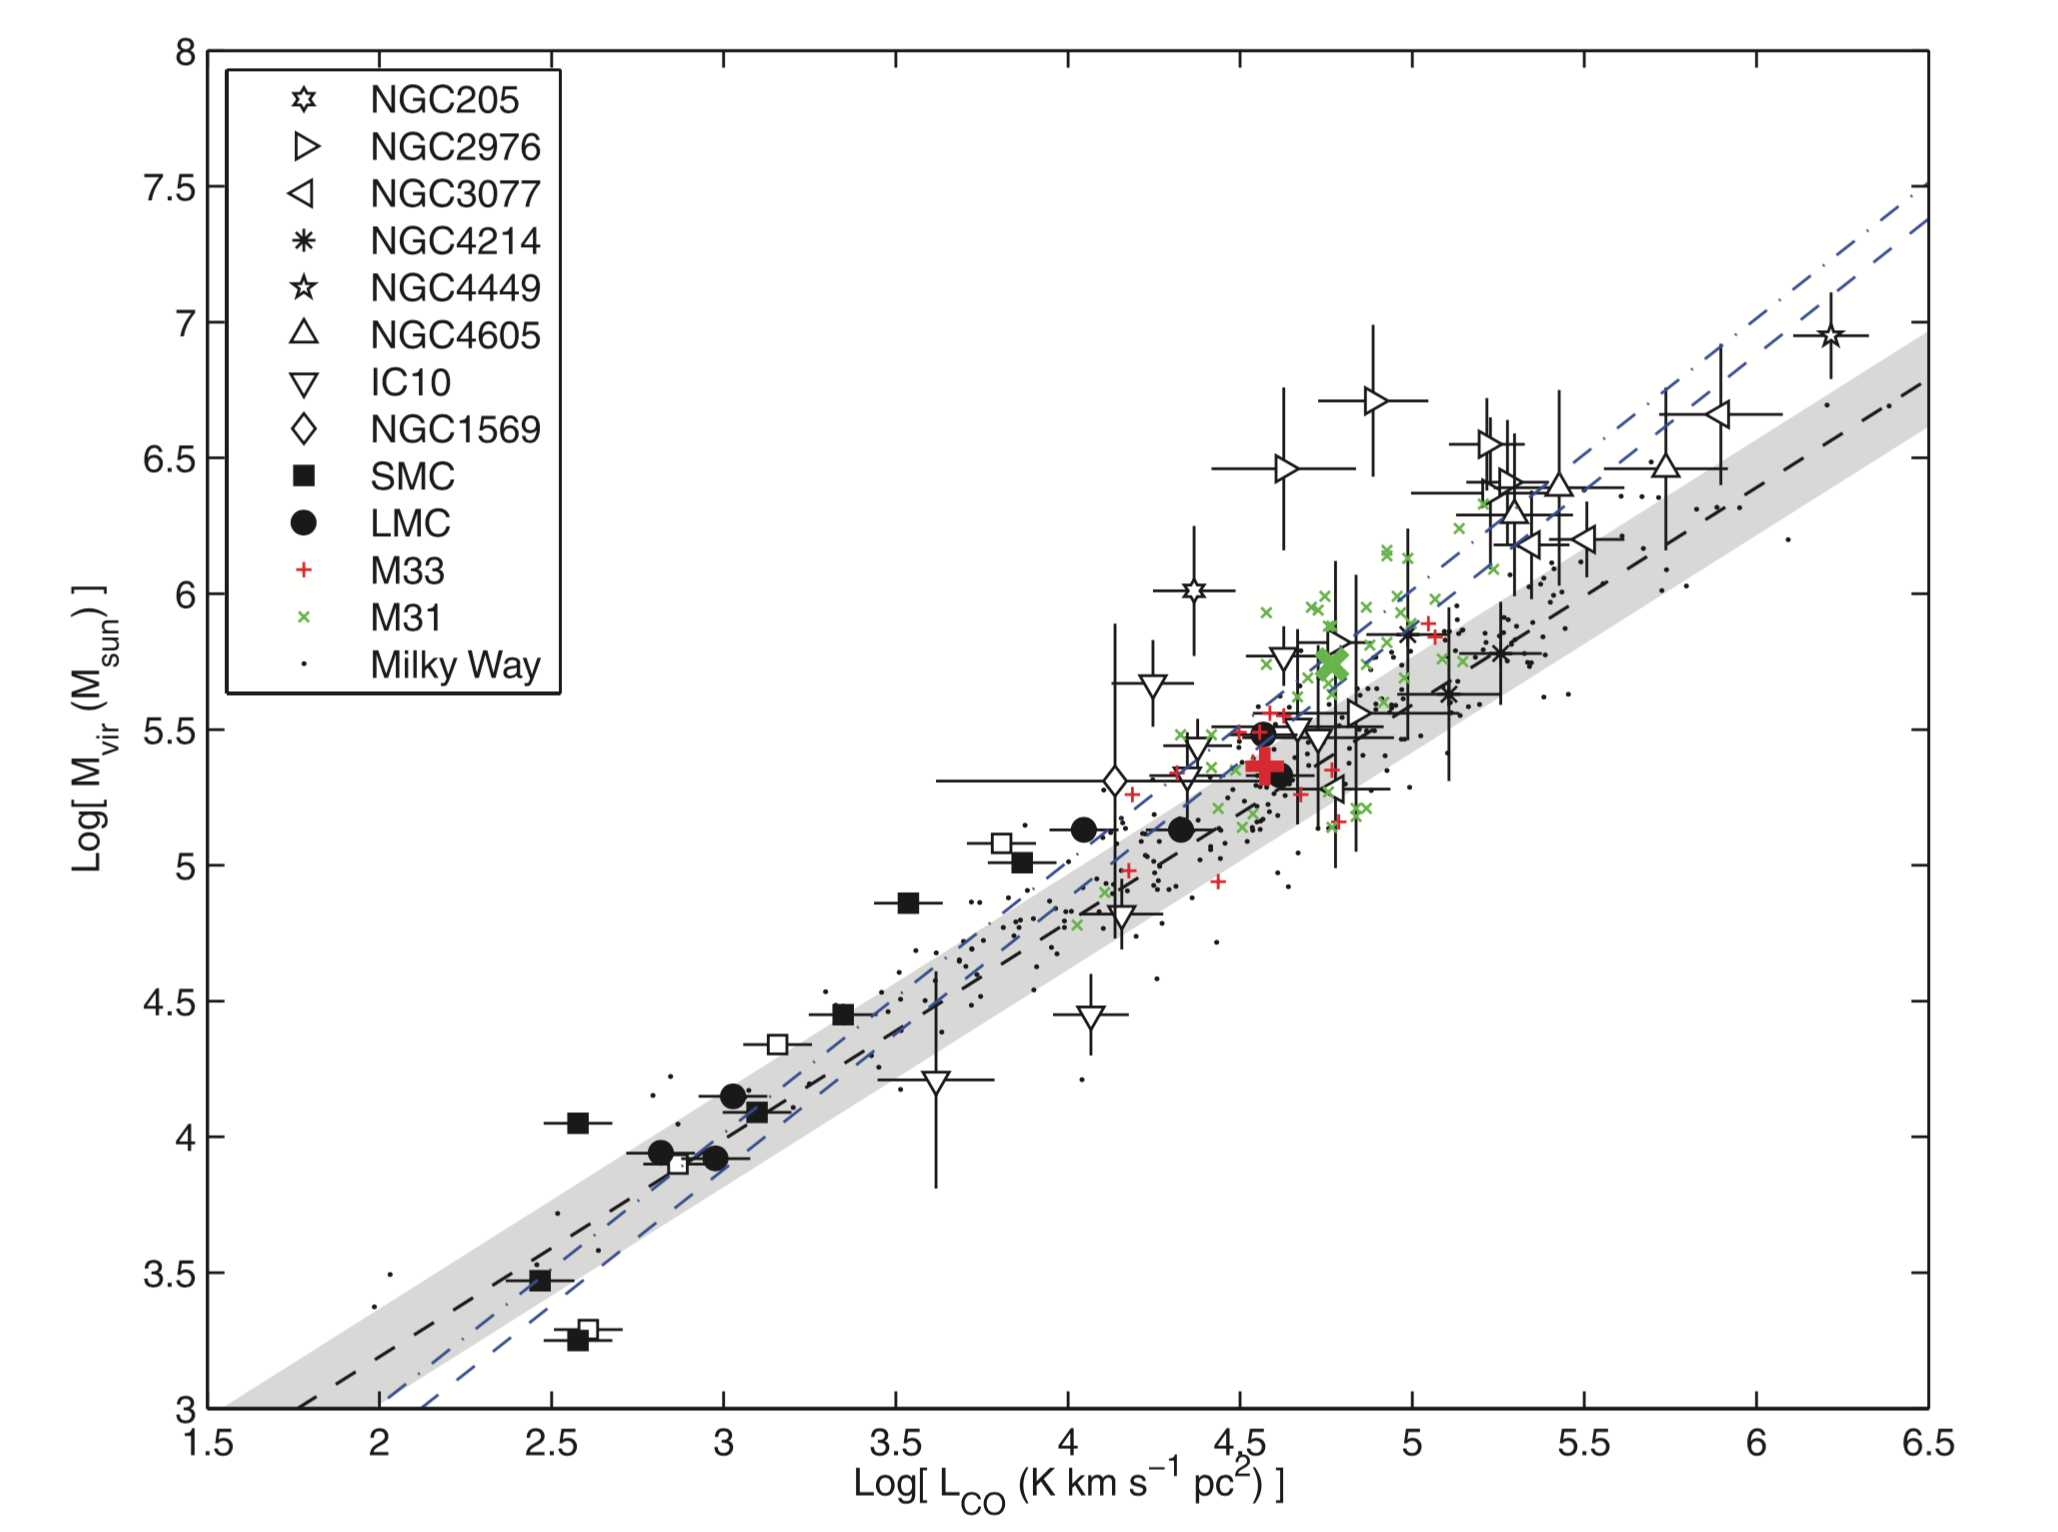
\includegraphics[width=16cm]{../image_intro/mvirial_lco.eps}
\caption{Relation between The Virial mass and CO luminosity for the Milky Way (dots), M33 (open circles), m31 (triangles), and IC 10 (squares) clouds. The Virial masses measured from selected high spatial resolution CO observations are shown. The extragalactic molecular clouds are very similar to those in the Milky Way. Adapted from \cite{Young91}}
\end{figure}
 

\subsubsection*{Neutral Gas}

Neutral hydrogen clouds are traced by 21-cm emission. The 21-cm emission comes from the fact that most of hydrogen in the ISM (excluding the regions close to type ``O" and ``B" stars) are in their ground state. The electron and proton spins in the ground state can be parallel (i.e. both spin up) or anti-parallel (i.e. proton's spin is up and electron's spin is down or vice versa). 

The energy state of anti-parallel mode is slightly less than parallel mode. Hence, electrons in the parallel mode have a tendency to flip to the anti-parallel mode (atoms always want to be in the state with lowest energy possible). Since the energy difference between these two states is small, eventually it takes millions of years before this transition happens. There are large amounts of atomic hydrogen in the ISM. Therefore, at any given time, there are enough hydrogen atoms that are emitting the 21-cm radiation, even though the transition is really rare. 

The density of the atomic hydrogen along the line-of-sight is proportional to the intensity of the 21-cm emission. Atomic hydrogens, that are along the line-of-sight contribute to the energy received. These properties make the 21-cm a very useful tool to study gas in the ISM and trace the large-scale distribution of galaxies in the universe (HI is detectable in most spiral galaxies and some elliptical galaxies). Although the 21-cm emission is the most reliable technique to map the ISM, the linear relationship between the intensity and the column density of the gas breaks down when the gas is optically thick \citep{Braun09}.

\subsubsection{Dust Emission as a Tracer of Gas}

Studying the gas cloud in the ISM of distant galaxies by using direct methods is almost impossible and not practical. \cite{Hildebran83} was the first person to suggest that one way to estimate the mass of the gas in the ISM might be from the optical depth of the sub-millimetre continuum emission from the dust; continuum dust emission is generally optically thin. The Herschel Space Telescope \cite{Pilbratt10} measured the continuum dust emission from hundreds of galaxies\citep{Eales10, Oliver12}. This amount of observational data provides a unique opportunity to study the ISM of galaxies using dust emission. 

 One of the advantages of using the dust emission as a tracer of the gas mass is that unlike the direct method, the high spatial resolution is not necessary anymore. The other important advantage is that this method solves the newly-found problem of the "dark gas"€™ in the galaxies. Dark gas is a significant fraction of the gas in the galaxy which is traced by neither the 21-cm emission nor the CO emission \citep{Abdo10}. So it is really hard to detect them by telescopes, but accurate gas to dust ratio can lead to an accurate estimate of dark gas mass in galaxies. 

There are many disadvantages regarding the use of the gas to dust ratio in the ISM. In order to use the dust as a tracer of the gas mass, first a relationship between the optical depth and the mass of the dust and then a relationship between the mass of the dust and the mass of the gas must be derived. \cite{Draine03} pointed out that this approach is uncertain because of the uncertainly in the radiative efficiency of dust grains. Also methods of measuring the gas to dust ratio in galaxies are not accurate, which means that there are problems in both steps \citep{Hildebran83}. Also by using current telescopes, it is difficult to detect dust emission from galaxies at z $>$ 0.1 \citep{Ealas12}. Besides, in some cases such as the Virgo cluster, dust mass is more tightly correlated with the total gas mass than to the masses of molecular or atomic gas separately \citep{Corbelli11}. 

In addition to all the disadvantages mentioned before, the dust method has two major practical problems: firstly, to apply this method, knowing the temperature of the dust is necessary. To solve this problem, measurement of the continuum emission at far-infrared wavelengths enough to cover the peak of the emission must be very accurate \citep{Ealas12}. The other problem is that there is evidence that the gas to dust ratio depends on the metallicity of the gas \citep{Lisenfeld98, Draine07}, but even in direct methods the dependence on metallicity must be solved. 

Certainly the gas to dust ratio as a tracer of the total gas in galaxies has a number of problems. Unfortunately, at present, given the available devices and technologies, we cannot reach a high-resolution that is sufficient to detect the gas cloud directly. Therefore, so far this method is the best available solution for measuring the total gas in distant galaxies. 



\subsection{Extinction and Attenuation}
\label{sec: ism}
In this section, dust ``attenuation" and ``extinction" will be introduced and their effects on measuring the SFR will be briefly discussed. More advanced and detailed discussions on this topic is out of the scope of this paper; and for more information one can refer to the review by \citep{Calzetti01}. 

Extinction happens when there is a combination of both absorption and scattering of radiation by dust. The distribution of the dust that lies between a source and the observer is irrelevant to the total extinction value because the source is a background point source (left panel of Fig.{~\ref{fig:duste}}).

Attenuation refers to the effect of dust with embedded light sources distributed throughout. The dust itself can be clumpy or smooth\citep{Calzetti13}. In this situation the relative location of the dust and light sources affect the net absorbed and scattered light, and that happens because both the light sources and the dust have extended distributions (right panel of Fig.{~\ref{fig:duste}}). Dust scattering's effect depends on whether it is in or out of the line of sight. When the dust is in the line of sight, attenuation will make the emerging light dimmer and the SED will be bluer. This is the typical situation that comes across when studying galaxies or extended regions within galaxies.

\begin{figure}[h]
\label{fig:duste}
\centering
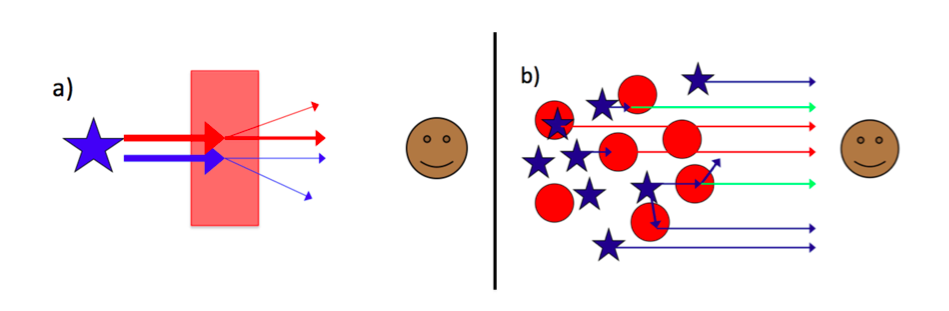
\includegraphics[width=16cm]{../image_intro/dustextinction}
\caption{The cartoon of: a) a point source behind a screen of dust, a typical situation to have an extinction; and b) the distribution of stars and clumps of dust, typical system, when attenuation effect is observed. Adopted from \cite{Calzetti13}}
\end{figure}

In order to describe the decrease in the intensity of the original beam when it passes through a region where dust particles are present while taking into account the radiation added to the beam by scattering into the line of sight, an integro-differential equation of the radiative transfer of light through dust is used. At UV/optical/near-IR wavelengths, the radiative transfer equation is:

\begin{equation}
\frac{dI_{\nu}}{d\tau} = -I_{\nu}  + \frac{a_{\nu}}{\pi} \int I_{\nu}\phi(\nu,\cos \Theta)d\Omega
\end{equation}
where I$_{\nu}$ is the intensity of radiation, $\tau$ is the dust's optical depth, a$_{\nu}$ is the dust albedo, which refers to the ratio of the scattering coefficient to the sum of the scattering and absorption coefficients. $\phi(\nu,\cos \Theta)$ is the scattering phase function, and $\Theta$ is the angle between the scattered photon and the line of sight. Both a$_{\nu}$ and $\phi(\nu,\cos \Theta)$ are described in more detail in \citep{Draine03}. The source function, i.e., the dust emission, which usually has small values for wavelengths shorter than a few $\mu$m is neglected in the equation above. This decrease in the intensity of the stellar radiation must be calculated and corrected for different emission; otherwise, it causes underestimation of the SFR. 


%%%%%%%%%%%%%%%%%%%%%%%%%%%%
%chapter :stellar mass
%%%%%%%%%%%%%%%%%%%%%%%%%%%%
\section{Stellar Mass}
\label{starmass}
One of the most fundamental physical parameters which describes the present state of the galaxies is stellar mass. It was pointed out that stellar mass is linked with the structure and star formation history of disc galaxies \citep{Gavvazi96} and all morphologies \citep{Scodeggio02}. In order to determine stellar population in spiral galaxies, the mean stellar mass density of a galaxy may be a more basic parameter than the total stellar mass \citep{Bell00}. \cite{Kauffmann03} tested that on more than 100,000 galaxies observed by Sloan Digital Sky Survey \citep[SDSS;][]{York00}. They also showed that these results are applied for all morphological types.

Measuring the mass of the stellar population is indirect and subject to significant uncertainties. In principle there are two ways to measure stellar mass in galaxies. First is measuring the dynamical mass of galaxies using kinematics \citep{Cappellari06} or lensing \citep{Auger09}, and then modelling the mass of the dark matter and subtracting it from the measured mass. This method has been successful to predict and subtract the mass of the dark matter, which is the dominant mass in galaxies \citep{Zaritsky94},  and can easily cause uncertainties as high as the order of the measurement. 

The second method is based on stellar population models \citep[e.g.][]{ Bruzual93, Kotulla09} and using them to connect stellar mass to an observable, like luminosity in different wavelengths, colours, spectral energy distribution from spectroscopy or multi-band observations. This method has uncertainties too, and one must also model the uncertainties. Uncertainties come from uncertainties in the stellar initial mass function (see section{~\ref{sec: imf}}), the stellar evolution models, especially the stage where they have most luminosity in their evolution, and the evolutionary state of galaxy \citep[see,][]{Dalcanton12}, and star formation histories. 

In order to translate between photometry and dynamics the stellar mass to light ratio (M/L) is needed. Measuring the accurate M/L can easily lead us to stellar mass surface density.  To do that, the M/L by can be measured using scale relation between them, from different colours and then multiply it by the surface brightness to calculate the local surface stellar mass density. The M/L scale relations make a connection between two methods of measuring stellar mass \citep{Bell03}. These relations are indirect methods for measuring the stellar masses and have high uncertainties in specific cases, but they help to study the stellar mass in large samples. This is one of the solution to the problem of the measuring the stellar mass within galaxies. As a result it is important to check the accuracy of total stellar mass estimations and provide methods, which measure and produce a map of the stellar mass surface density distribution in galaxies. This method gives more accurate result than measuring the stellar mass surface density distribution from single-band images rescaled by uniform mass to light ratio \cite{Zibetti09}.
 
Having two independent methods to measure stellar mass helps to compare the results and check whether there are any systematic differences. Comparing the results from measuring stellar mass in stellar clusters shows there is no huge difference. Comparing the results from measuring stellar mass within galaxies shows that the deferences are on the order of a few x10 percent, so one should be more careful to model subtleties \citep{McLaughlin05}. In the following we address the approaches of measuring stellar mass in galaxies in more detail.

\subsection{Dynamical Mass}
The mass distribution in disk galaxies is usually calculated from rotation curves or integrated line profiles from emission lines such as H${\alpha}$, CO, and HI lines. Thanks to the current generation of detectors, the H$\alpha$ and CO lines have very high-resolution spectra over most of the optical disk, and cover most regions in the sky. Integrated line widths only yield an estimate of a total mass within some (uncertain) isophotal radius.

Resolved rotation curves produced from H$\alpha$, HI and CO lines are proportional to optical emission lines within the optical disk of galaxies, \citep{Courteau13} which helps us to measure the rotational curves. The simplest way to estimate the mass of a galaxy is assuming that the physics of the galaxy is the simple Newtonian physics. Therefore, the Mass within a potential $\phi$ and the circular velocity in the spherical system is given by:
\begin{equation}
\label{eq: simpmass}
V^2_{circ}(r)=r\frac{d\phi}{dr} = G\frac{M(r)}{r}
\end{equation}
where $M(r)$ is the mass within a sphere of radius $r$. For a flattened disk which is the case in most spiral galaxies, the right hand side of equation {~\ref{eq: simpmass}}  must  be replaced by the more exact expression derived by \cite{Freeman70}. He assumed in case of no dark matter or bulge, the rotation curve of a self-gravitating disk is:
\begin{equation}
V^2_{circ}(R)= 4\pi G \Sigma_{0}R_{d} y^2[I_0(y)K_0(y) - I_1(y)K_1(y)]
\end{equation}
where $G$ is the gravitational constant, $\Sigma_0$ the central surface brightness, $R_d$ the disk scale length, $4y=\frac{R}{2R_d}$, and $I_i(y)$ and $K_i(y)$ are the first and second kind of modified Bessel functions.

Describing more about calculating dynamical masses in galaxies is beyond the scope of this paper. Just note that methods mentioned above is the first order of approximation. For more accurate result one should consider that the rotational velocity is not circular and the fact that galaxies contain millions of stars plus interstellar objects therefore simple two object Newtonian physics is not the case here. There are lots of different profiles to fit the rotation curve for galaxies. A detailed review of dynamical mass of galaxies can be found in Courteau et al review paper (2013).

\subsection{Stellar Population Method}
Galaxies can be observed because of their stellar emission and stars radiate the energy produced from nuclear reactions in their cores. Given the star's initial mass, the theory of stellar evolution can describe the amount of energy released. Hence, stellar mass that is responsible for radiation of stars can be derived by modelling the spectral energy distribution of galaxies. However, there is a fraction of mass of evolved stars which no longer emit radiation yet still contribute to the galaxy mass as stellar remnants. 

As mentioned before, stellar population synthesis models is used to reproduce the SED of a stellar population using many physical parameters. These parameters, which control the time evolution of the stellar population are:
the age, $t$, of the population, measured in years, also referred to the time passed since the star formation was began;
the star formation history (SFH), often parametrized with SFR $\propto e^{-1/\tau}$; the IM; The metallicity, which is calculated as the ratio of abundance Z of elements heavier than He to abundance of H ([Z/H]), or as ratio of abundance of iron ([Fe/H]); 
and the chemical composition ratios, or the fraction of all key elements in galaxies and those values measured in the Sun. The stellar evolutionary tracks, the stellar spectral libraries, the parametrization for the mass-loss which affects several late stages of evolution are necessary for stars placing at specific evolutionary phases \citep{Courteau13}.


%\subsubsection{Calibration light of stars} 
The basic idea behind the finding the suitable calibration between flux/luminosity of the stars in different wavelengths and stellar mass is that one can use the SFHs recovered from synthesizing the stellar optical CMs in different regions in the galaxies. The calculated stellar mass can be used  to calibrate the fluxes from the stars as the easily measurable parameters of stars. Using NIR bands, different groups tried to make a map of stellar mass distributions within galaxies \citep[e.g.,][]{Elmgreen84}.  Using $B-V$ colours \citep{Bell01} and $Spitzer$ 3.6- and 4.5-$\mu$m, M/L correction, \cite{Kendall08} produced stellar mass surface densities of M81. 

\cite{Zibetti08} suggested for reaching the maximum spatial resolution one can recombine the photometric information on a pixel-by-pixel study \citep{Conti03}. They used this method to study the stellar mass distribution in galaxies as well as the dependence of the SED on stellar mass density. To do so the surface density of stellar mass is derived by 
\begin{equation}
\label{equ: massphot}
\Sigma M_\star (\alpha, \delta) = \Sigma \lambda(\alpha, \delta) \gamma_{\lambda}(\alpha, \delta)
\end{equation}
where $\Sigma \lambda(\alpha, \delta)$ is the surface brightness and $\gamma_{\lambda}(\alpha, \delta)$ is the effective stellar M/L in an effective wavelength $\lambda$. In equation~\ref{equ: massphot},  $\gamma_{\lambda}$ can be described as a function of one or more colours as observed at the specified location in galaxy. Equation~\ref{equ: massphot} can be used for each position in a galaxy.


\cite{Eskew12} related easily observable quantities to the stellar mass. They used 3.6$\mu$m and 4.5$\mu$m fluxes  for calibration of the stellar mass, because these two bandpasses are almost insensitive to the emission from young stellar population, dust absorption and emission. Also thanks to $Spitzer$ and WISE \citep{Wright10} telescopes, great amount of data from many regions in the sky is available, in these bands, which help to test them on more regions and have a more accurate calibration. They also test the 3.6- and 4.5 $\mu$m fluxes as proxies for stellar mass in the Large Magellanic Cloud and find the empirical relation between mass of the stars and the luminosities of stars as below:

\begin{equation}
\label{equ:eskew}
M = 31.84 \times 10^{5.65} L_{3.6}^{2.85} L_{4.5}^{-1.85}
\end{equation}

where M$_{\star}$ is the stellar mass and $L = \nu L_{\nu}[\lambda]$ is the luminosity in erg/s/$\AA$.
 
\cite{Zhu10} used the SDSS and the $Spitzer$ Wide-area Infrared Extragalactic Survey \citep[SWIRE;][] {Lonsdale03} to find the calibration between luminosity of the galaxies and stellar masses. Using the M/L of galaxies, they found the correlation between $K_s$ band, $3.6 \mu$m and $4.5 \mu$m band luminosities and stellar masses and formulate these correlations as:
\begin{align}
\label{equ: zhu1}
\log M_{\star} = (-1.60 ) + (1.12)\times \log \nu L_{\nu}[K_s]\\
\log M_{\star} = (-0.79) + (1.19)\times \log \nu L_{\nu}[3.6\mu \rm m]\\
\label{equ: zhu3}
\log M_{\star} = (-0.25) + (1.15)\times \log \nu L_{\nu}[4.5\mu \rm m] 
\end{align}
where M$_{\star}$ is the stellar mass and $ \nu L_{\nu}[\lambda]$ is the luminosity in erg/s in specified wavelength. 

Measuring the stellar mass from equation~\ref{equ:eskew} is limited to the nearby galaxies, and might break down for high star forming regions, moreover, this equation have not tested on regions with different metallicity. Thus there is no calibration regarding variation in  metallicity \citep{Eskew12}. On the other hand equations~\ref{equ: zhu1} -~\ref{equ: zhu3} have been derived from a large sample of galaxies, and was tested on different type of regions and galaxies. Beside they can be used for more distanced galaxy as well as nearby galaxies \citep{Zhu10}. 

%%%%%%%%%%%%%%%%%%%%%%%%%%%%
%chapter: KS law
%%%%%%%%%%%%%%%%%%%%%%%%%%%%

\section{Scaling the SFR Using Schmidt-Kennicut Law}

The first idea about scaling the star formation rate on the galaxy scale was proposed as a connection between the total star formation rate and the mass of interstellar gas. \cite{Schmidt59} assumed the constant IMF of stars, $\Psi (M)$, a stellar lifetime function {$T(M$)}, and a star formation rate {$SFR(T)$} and derived the star formation rate (SFR) over the history of the Milky Way. He scaled SFR with a power {\it n} of the gas mass, $M_{gas}$. Then $SFR(T)\Sigma_{M}(M) = c[M_{gas}(t)]^n$, for a summation over all stellar type $M$. A power law relation between surface densities of star formation and gas is known as the Schmidt law and is written as:
\begin{equation}
\Sigma_{SFR} \propto \Sigma_{gas}^n
\end{equation}
where $\Sigma_{SFR}$ is surface density of star formation, $\Sigma_{gas}$ is the surface density of gas in a galaxy and, {\it n} is the power index.

Following \cite{Schmidt59}, many groups worked on the scaling relation between the surface density of star formation, and the surface density of gas. \cite{Buat89} assumed the constant H$_2$/CO ratio and a \cite{Scalo86} initial mass function for the Milky Way. They measured SFR from the UV flux corrected and included molecular and atomic gas to derive the correlation between the star formation rate and the gas surface density. Another major work in that year was \cite{Kennicutt89}. By using H$\alpha$ emission for star formation, and HI and CO as a tracer of gas with constant H$_2$/CO, for more than 15 galaxies, he determined the average H$\alpha$ flux can be scaled with the average gas surface density to a power between 1 and 2.  To get better results he calculated star formation rate both as a function of galactocentric radius and averaged over whole galaxy disks. He also showed that the correlation is more accurate with using only HI as a tracer of gas. 

A decade later, \cite{Kennicutt98a} examined another group of galaxies. He used H$\alpha$, HI and CO observations of 61 normal spiral galaxies and 36 starburst galaxies and showed that the disk-average SFRs and gas densities for this samples are well represented by the Schmidt law with the power of $1.4 \pm 0.15$. Using this power index, the Schmidt law can be rewritten as:

\begin{equation}
\Sigma_{SFR} \propto \Sigma_{gas}^{1.4\pm0.15}
\end{equation}
which is often referred to as the Kennicutt-Schmidt (KS) law. 

In more recent studies, \cite{Kennicutt08} investigated the local star formation law in M51 with 0.5-2 kpc resolution. For the SFR he used pa${\alpha}$ and $24\mu$m + H${\alpha}$ lines and for gas density he used constant conversion factor for CO to H$_2$. He found a correlation, from the radial variation of both SFR and gas surface density, with an index of $1.56 \pm 0.04$. He could not find any correlation between SFR and HI only clouds, but the correlation with the molecular cloud was about the same as the total gas.
It should be noted that the KS law can not be applied for the whole range of gas densities. In parallel studies, the star formation threshold was introduced and it was pointed out that calculated SFR is much lower than the value predicted by the KS law at low gas densities $( < 1-10\sim$ M$_{\odot}$ pc$^{-2})$ e.g. in regions far outside the optical disk \citep[e.g.,][]{Martin01, Bigiel08}

The Schmidt-Kennicutt scaling relation for star formation is valid for different types of galaxies both in the local universe \citep[e.g.,][]{Kennicutt98a, Bigiel08} and at high-Z \citep[e.g.,][]{Genzel10}, but it is strange that they only consider the effect of gas component while in reality various ISM and stellar objects affect the processes of formation of stars. Current proposed Schmidt relations, do not include the effects of metallicity \citep{Gnedin10}, dust grains, radiation shielding of H$_2$ regions \citep[for a review, see][]{Hollenbach99}, and stellar gravitational effects, as they only invoke the gas component.  Existing stars which form over the whole galaxy's life time are the reason for many of the processes mentioned above. As an example the gas angular momentum can be removed or nuclear SFRs can be increased by the gravitational effects of stellar bars in normal galaxies \citep[e.g.,][]{Sersic67}.  

\cite{Hunter98} have shown that, in low surface brightness galaxies the SFR density is only related to the stellar mass density. Also similar relations between stellar masses and SFR densities are seen within galaxies by \cite{Ryder94}, \cite{Hunter04} and recently by \cite{Leroy08} for specific galaxy types or limited density ranges. \cite{Shi11} found a tight relationship between stellar mass surface density, SFR and gas surface density by studying on a large sample of galaxies. They showed this relation as a power law relation and referred to it as the extended Schmidt law: 

\begin{equation}
\Sigma_{SFR} \propto \Sigma_{gas}^{\alpha} \Sigma_{star}^{\beta}
\end{equation}
where $\Sigma_{SFR}$ is SFR surface density, $\Sigma_{gas}$ and $\Sigma_{star}$ are gas mass and stellar surface density. $\alpha$ and $\beta$ are the power law indexes.  They showed that this relation not only predicts SFR as well as the KS law for galaxies and spatially resolved regions ($\sim$1 kpc sizes) where the KS law works, but also is acceptable for low surface brightness galaxies and regions where the KS law fails.

\begin{figure}[h]
\label{fig:duste}
\centering
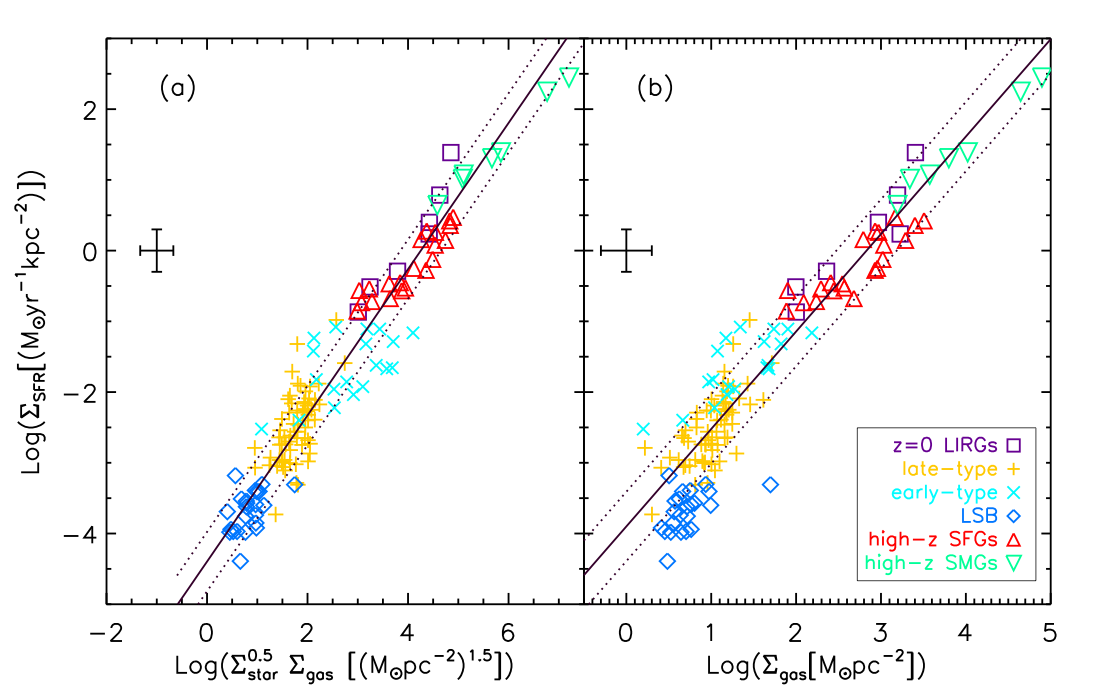
\includegraphics[width=16cm]{../image_intro/schmidtvsextended}
\caption{Comparing The extended Schmidt law (a) and the Kennicutt-Schmidt relationship (b) for predicting the SFR. The solid and dotted lines are the best fit and observed 1-$\sigma$ scatter, respectively. The fit to the KS law (right panel) is done excluding LSB and early type galaxies. Adapted from \cite{Shi11}.}
\end{figure}


%%%%%%%%%%%%%%%%%%%%%%%%%%%%
%chapter: current work
%%%%%%%%%%%%%%%%%%%%%%%%%%%%
\section{Current issues and the Present Project}
\label{chap:mp}
Studying formation of stars helps us understand the formation and evolution of the universe. Since forming stars contains many complex physical processes, theoretical studies cannot yet give a complete picture of star formation. Therefore empirical studies are used to find scaling laws indicating, which parameters have effects on star formation. Between different scaling relations for star formation, the KS law is the most tested empirical star formation law. Since 1959, many studies have tested KS law on regions inside the Milky Way, nearby galaxies and high redshift galaxies. Not only observational studies, but also  simulations both apply and investigate KS law. Despite all these studies, there are still many unsolved questions about the KS law; Is it really a good correlation? What is the slope, and is it unique?, Does SFR surface density only scale with gas density? does the scatter affect by a second parameter(s)? What is the limit for applying the KS law? Is the SFR surface density correlation with total gas density stranger than with the H$_2$ surface density alone?

Many groups are studying the KS law from different approaches to answer the questions listed in above. The extended Schmidt law is a newer version of the KS law, which by considering the effect of old stellar population on the SFR provides stronger correlation for the SFR than the other scaling laws. Although in original paper this law is tested on large sample of various types of galaxies, but further studies are necessary, due to the fact that this law is tested on the total SFR and not on different regions on galaxies to determine effect of environment on the SFR. In this project, the extended version of the Schmidt law will be tested on the Andromeda galaxy using both pixel by pixel relation and radial average along the disk. To due so star formation rate will be measured using equations~\ref{equ: halphaplus24} and ~\ref{sfr_tot_IR}. In order to find the gas surface density, direct method to map the ISM is chosen. Stellar surface density will be calculated by calibrations from both \cite{Eskew12} and \cite{Zhu10}.

The Andromeda galaxy is chosen for this project due to its similarity in the structure to the MW. Also it is the nearest spiral galaxy and provides a clear image of a galaxy like our own with the advantage that we get a "€œglobal"€ picture, whereas, studies of the MW are limited by our location within the Galaxy.  The Andromeda is closest spiral galaxy to the MW, therefore, we can have higher resolution images of it than we have of any other spiral galaxy. Having high resolution images provides us data from different regions within the galaxy with different physical situations (e.g. metallicity, surface brightness and etc.). All these parameters make the Andromeda a suitable test bed for studying the scaling law. The KS law has been tested on the Andromeda galaxy many times but the results have been controversial. The range of slope of KS law calculated for the Andromeda galaxy is between 0.5 - 2 \citep[e.g.,][]{Tabatabaei10, Ford13}. Testing extended Schmidt law on the Andromeda galaxy would help us recognise parameters that affect the star formation in the Andromeda galaxy and leads us to model and simulate star formation more accurately. Also it helps us answer questions about in what types of the regions (e.g. in case of different surface brightness, metallicity, distance from the disk, etc.) effect of the stellar mass is more important.